\documentclass[acmsmall,screen,review,anonymous]{acmart}
\usepackage{bbm}
\usepackage{ebproof}
\usepackage{minted}
\usepackage{tikz-cd}
\usepackage{subcaption}

\bibliographystyle{ACM-Reference-Format}
\citestyle{acmauthoryear}

% Notations
\newcommand{\kw}[1]{\ensuremath{ \mathsf{#1} }}
\newcommand{\ifr}[1]{\mathrel{[{#1}]}}
\newcommand{\que}{\circ}
\newcommand{\ans}{\bullet}
\newcommand{\vref}{\le_\kw{v}}
\newcommand{\mext}{\le_\kw{m}}
\newcommand{\refby}{\preceq}
\newcommand{\scref}{\sqsupseteq}
\newcommand{\screfd}{\sqsubseteq}
\newcommand{\unitset}{\mathds{1}}
\renewcommand{\preceq}{\preccurlyeq}
\newcommand{\intl}[1]{\underline{#1}}

% Names of things
\newcommand{\ClightP}{\ensuremath{\mathsf{Clight+}}}


\title{Compositional Compiler Correctness with Encapsulated State}

\begin{document}

\maketitle

\newpage
\tableofcontents
\newpage

\section{Introduction} %{{{

There are many verification frameworks based on CompCert,
but none of them support encapsulated state.
At most, permissions,
but here the context still ``sees'' the memory,
even though it must be shown to be insensitive to it.

We do better.

%}}}

\begin{figure} %{{{
  \textbf{Notations}
  \\[1em]
  \begin{tabular}{llcllc}
    Basic component & Def.~\ref{def:lts} &
    $L : A \twoheadrightarrow B$ &
    Stateful component & Def.~\ref{def:slts} &
    $\Sigma : A \rightarrow B$
    \\
    Basic convention & Def.~\ref{def:simconv} &
    $\mathbb{R} : A^\sharp \Leftrightarrow A^\flat$ &
    Stateful convention & Def.~\ref{def:sconv} &
    $\mathbf{R} : A^\sharp \leftrightarrow A^\flat$
    \\
    Basic simulation & Def.~\ref{def:sim} &
    $L^\sharp \le_{\mathbb{R}_A \twoheadrightarrow \mathbb{R}_B} L^\flat$ &
    Stateful simulation & Def.~\ref{def:ssim} &
    $\Sigma^\sharp \preceq_{\mathbf{R}_A \rightarrow \mathbf{R}_B} \Sigma^\flat$
  \end{tabular}
  \\[1em]
  \textbf{Layered composition}
  \\[1em]
  \begin{tabular}{cc@{\qquad}cc}
    Def.~\ref{def:lcomp} &
  {$\begin{prooftree}
      \hypo{L_1 : B \twoheadrightarrow C}
      \hypo{L_2 : A \twoheadrightarrow B}
      \infer2{L_1 \odot L_2 : A \twoheadrightarrow C}
    \end{prooftree}$}
    &
    Def.~\ref{def:slcomp} &
  {$\begin{prooftree}
      \hypo{\Sigma_1 : B \rightarrow C}
      \hypo{\Sigma_2 : A \rightarrow B}
      \infer2{\Sigma_1 \circ \Sigma_2 : A \rightarrow C}
    \end{prooftree}$}
    \vspace{1em} \\
    Thm.~\ref{thm:lcompsim} &
  {$\begin{prooftree}
      \hypo{L_1^\sharp
            \le_{\mathbb{R}_B \twoheadrightarrow \mathbb{R}_C}
            L_1^\flat}
      \hypo{L_2^\sharp
            \le_{\mathbb{R}_A \twoheadrightarrow \mathbb{R}_B}
            L_2^\flat}
      \infer2{L_1^\sharp \odot L_2^\sharp
            \le_{\mathbb{R}_A \twoheadrightarrow \mathbb{R}_C}
            L_1^\flat \odot L_1^\flat}
    \end{prooftree}$} &
    Thm.~\ref{thm:slcompsim} &
  {$\begin{prooftree}
      \hypo{\Sigma_1^\sharp
            \preceq_{\mathbf{R}_B \rightarrow \mathbf{R}_C}
            \Sigma_1^\flat}
      \hypo{\Sigma_2^\sharp
            \preceq_{\mathbf{R}_A \rightarrow \mathbf{R}_B}
            \Sigma_2^\flat}
      \infer2{\Sigma_1^\sharp \circ \Sigma_2^\sharp
            \preceq_{\mathbf{R}_A \rightarrow \mathbf{R}_C}
            \Sigma_1^\flat \circ \Sigma_1^\flat}
    \end{prooftree}$}
  \end{tabular}
  \\[1em]
  \textbf{Vertical composition}
  \\[1em]
  \begin{tabular}{cc@{\qquad}cc}
    Def.~\ref{def:ccomp} & {$
    \begin{prooftree}
      \hypo{\mathbb{R} : A^\sharp \Leftrightarrow A^\natural}
      \hypo{\mathbb{S} : A^\natural \Leftrightarrow A^\flat}
      \infer2{\mathbb{R} \cdot \mathbb{S} : A^\sharp \Leftrightarrow A^\flat}
    \end{prooftree}
    $} &
    Def.~\ref{def:sccomp} & {$
    \begin{prooftree}
      \hypo{\mathbf{R} : A^\sharp \leftrightarrow A^\natural}
      \hypo{\mathbf{S} : A^\natural \leftrightarrow A^\flat}
      \infer2{\mathbf{R} \mathbin; \mathbf{S} : A^\sharp \leftrightarrow A^\flat}
    \end{prooftree}
    $}
    \vspace{1em} \\
    Thm.~\ref{thm:vcomp} & {$
    \begin{prooftree}
      \hypo{L^\sharp
        \le_{\mathbb{R}_A \twoheadrightarrow \mathbb{R}_B}
        L^\natural}
      \hypo{L^\natural
        \le_{\mathbb{S}_A \twoheadrightarrow \mathbb{S}_B}
        L^\flat}
      \infer2{L^\sharp
        \le_{\mathbb{R}_A \cdot \mathbb{S}_A \twoheadrightarrow
             \mathbb{R}_B \cdot \mathbb{S}_B}
        L^\flat}
    \end{prooftree}
    $} &
    Thm.~\ref{thm:svcomp} & {$
    \begin{prooftree}
      \hypo{\Sigma^\sharp
        \preceq_{\mathbf{R}_A \twoheadrightarrow \mathbf{R}_B}
        \Sigma^\natural}
      \hypo{\Sigma^\natural
        \preceq_{\mathbf{S}_A \twoheadrightarrow \mathbf{S}_B}
        \Sigma^\flat}
      \infer2{\Sigma^\sharp
        \preceq_{\mathbf{R}_A \mathbin; \mathbf{S}_A \twoheadrightarrow
             \mathbf{R}_B \mathbin; \mathbf{S}_B}
        \Sigma^\flat}
    \end{prooftree}
    $}
  \end{tabular}
  \\[1em]
  \textbf{Adjoining explicit state}
  \\[1em]
  \begin{tabular}{cc@{\qquad}cc}
    Def.~\ref{def:lift} &
    {$
    \begin{prooftree}
      \hypo{L : A \twoheadrightarrow B}
      \infer1{L@K : A@K \twoheadrightarrow B@K}
    \end{prooftree}
    $} &
    Def.~\ref{def:slift} &
    {$
    \begin{prooftree}
      \hypo{\Sigma : A \rightarrow B}
      \infer1{\Sigma@K : A@K \rightarrow B@K}
    \end{prooftree}
    $}
    \vspace{1em} \\
    & &
    Def.~\ref{def:liftsconv} &
    {$
    \begin{prooftree}
      \hypo{\mathbf{R} : A^\sharp \leftrightarrow A^\flat}
      \infer1{\mathbf{R}@\langle K^\sharp, K^\flat \rangle :
        A^\sharp@K^\sharp \leftrightarrow A^\flat@K^\flat}
    \end{prooftree}
    $}
    \vspace{1em} \\
    & &
    Thm.~\ref{thm:liftssim} &
    {$
    \begin{prooftree}
      \hypo{\Sigma^\sharp
        \preceq_{\mathbf{R}_A \rightarrow \mathbf{R}_B}
        \Sigma^\flat}
      \infer1{\Sigma^\sharp@K^\sharp
        \preceq_{\mathbf{R}_A@\langle K^\sharp, K^\flat \rangle \rightarrow
                 \mathbf{R}_B@\langle K^\sharp, K^\flat \rangle}
        \Sigma^\flat@K^\flat}
    \end{prooftree}
    $}
  \end{tabular}
  \\[1em]
  \textbf{Embedding simple components}
  \[
    \begin{prooftree}
      \hypo{L : A \twoheadrightarrow B}
      \infer1{\&L : A \rightarrow B}
    \end{prooftree}
    \qquad
    \begin{prooftree}
      \hypo{\mathbb{R} : A^\sharp \Leftrightarrow A^\flat}
      \infer1{\&\mathbb{R} : A^\sharp \leftrightarrow A^\flat}
    \end{prooftree}
    \qquad
    \begin{array}{c}
      \&(L_1 \odot L_2) \equiv \&L_1 \circ \&L_2
      \\[1ex]
      \&(\mathbb{R} \cdot \mathbb{S}) \equiv
        \&\mathbb{R} \mathbin; \&\mathbb{S}
    \end{array}
    \qquad
    \begin{prooftree}
      \hypo{L^\sharp
        \le_{\mathbb{R}_A \twoheadrightarrow \mathbb{R}_B}
        L^\flat}
      \infer1{\&L^\sharp
        \preceq_{\&\mathbb{R}_A \rightarrow \&\mathbb{R}_B}
        \&L^\flat}
    \end{prooftree}
  \]
  \\[1em]
  \textbf{Encapsulating state}
  \[
    \begin{prooftree}
      \hypo{\Sigma : A \rightarrow B@K}
      \infer1{\kw{fbk}_K(\Sigma) : A \rightarrow B}
    \end{prooftree}
    \qquad
    \begin{prooftree}
      \hypo{\Sigma^\sharp
        \preceq_{\mathbf{R}_A \rightarrow
                 \mathbf{R}_B@\langle K^\sharp,K^\flat \rangle}
        \Sigma^\flat}
      \infer1{\kw{fbk}_{K^\sharp}(\Sigma^\sharp)
        \preceq_{\mathbf{R}_A \rightarrow \mathbf{R}_B}
        \kw{fbk}_{K^\flat}(\Sigma^\flat)}
    \end{prooftree}
    \qquad
    \kw{fbk}_\mathbbm{1}(\Sigma) \equiv \Sigma
  \]
  \vspace{1ex}
  \[
    \kw{fbk}_{K_1}(\Sigma_1) \circ \kw{fbk}_{K_2}(\Sigma_2) \equiv
    \kw{fbk}_{K_1 \times K_2}(\Sigma_1@K_2 \circ \Sigma_2)
  \]
  \caption{Summary of key notations, definitions and properties}
    %Constructions on the left-hand side operate in terms of
    %the original semantic framework of CompCertO.
    %We extend that framework
    %to account for persistent encapsulated state,
    %shown on the right.
    %Construction which enable the manipulation of
    %encapsulated state are shown at the bottom.}
  \label{fig:overview}
\end{figure}
%}}}

\begin{figure} % fig:code {{{
  \centering\footnotesize
  \begin{subfigure}{0.45\textwidth}
\begin{minted}{C}
/* Encapsulated state */
static int c1, c2;
static V buf[N];

/* Accessors */
int inc1() { int i = c1++; c1 %= N; return i; }
int inc2() { int i = c2++; c2 %= N; return i; }
V get(int i) { return buf[i]; }
void set(int i, V val) { buf[i] = val; }
\end{minted}
  \subcaption{The translation unit $\kw{rb.c}$}
  \label{fig:rb}
  \end{subfigure}
  \hspace{4em}
  \begin{subfigure}{0.38\textwidth}
\begin{minted}{C}
/* Underlay signature */
extern int inc1(void);
extern int inc2(void);
extern V get(int i);
extern void set(int i, V val);

/* Layer implementation */
void enq(V val) { set(inc2(), val); }
V deq() { return get(inc1()); }
\end{minted}
  \subcaption{The translation unit $\kw{bq.c}$}
  \label{fig:bq}
  \end{subfigure}
  \caption{Running example, consisting of two C components.
    The component $\kw{rb.c}$
    implements a ring buffer by encapsulating an array
    and two counters. It is used by the component
    $\kw{bq.c}$ to implement a
    bounded queue.}
  \label{fig:code}
%\caption{The state of a ring buffer,
%  made of two counters and a fixed-size array,
%  is encapsulated behind a simple interface.}
%\label{fig:rb}
%\caption{This component relies on the ring buffer primitives
%  provided in Fig.~\ref{fig:rb} to implement a bounded-size queue.}
%\label{fig:bq}
\end{figure}
%}}}

\section{Basic framework} %{{{

We start our exposition by
describing the semantic model
used in CompCertO,
which will we use as a starting point
in our treatment of encapsulated state.
In \S\ref{sec:basic:compcertO}
we summarize the model as described by
\citet{compcerto}.
We then introduce new constructions
which will be used in our development,
namely layered composition (\S\ref{sec:basic:lcomp}) and
state annotations (\S\ref{sec:basic:state}).

The high-level structure of these constructions
is shown on the left-hand side of \autoref{fig:overview}.

\subsection{Semantics in CompCertO} \label{sec:basic:compcerto} %{{{

The compositional semantics of CompCertO uses %revolves around
a notion of open transition system $L : A \twoheadrightarrow B$.
The type $A \twoheadrightarrow B$ involves
two \emph{language interfaces} $A$ and $B$,
which decribe how components interact at various levels of abstraction
from C to assembly language.

\begin{definition} \label{def:li}
A language interface $A = \langle A^\que, A^\ans \rangle$
consists of a set of questions $A^\que$ and a set of answers $A^\ans$.
\end{definition}

Language interfaces specify the information exchanged between
a component and its environment
when control switches between the two.
Questions correspond to function invocations
and answers correspond to the function returning.
An execution of the component $L : A \twoheadrightarrow B$
is initiated with a question $q \in B^\que$
and terminates with a corresponding answer $r \in B^\ans$.
At any point during the execution,
$L$ may ask a question $m \in A^\que$ (an external call),
in which case it is suspended until an answer $n \in A^\ans$
resumes the execution.

As in the original CompCert semantics,
a transition system
executes by updating an internal state,
which is not directly observable
in its interactions with the environment.

\begin{definition}[Basic Component] \label{def:lts}
A basic component $L : A \twoheadrightarrow B$
is a tuple $L = \langle S, {\rightarrow}, I, X, Y, F \rangle$
consisting of:
\begin{itemize}
  \item a set $S$ of states;
  \item a transition relation ${\rightarrow} \subseteq S \times S$;
  \item a relation $I \subseteq B^\que \times S$
    which assigns possible \emph{initial states}
    to each question of $B$;
  \item a relation $F \subseteq S \times B^\ans$
    which specifies \emph{final states} together with
    corresponding answers in $B$;
  \item a relation $X \subseteq S \times A^\que$
    which identifies \emph{external states} and
    corresponding questions of $A$;
  \item a relation $Y \subseteq S \times A^\ans \times S$,
    which identifies \emph{resumption states}.
\end{itemize}
We write $n \mathrel{Y^s} s'$ when $(s, n, s') \in Y$.
This means that
after an external state $s$ triggers a question $m \in A^\que$ ($s \mathrel{X} m$),
and the environment replies with an answer $n \in A^\ans$,
the execution can resume with state $s'$.
\end{definition}

When $L : A \twoheadrightarrow B$
performs an external call in $A$,
the internal state $s$ is preserved
until an answer resumes the execution.
Note however that
no state is preserved across different executions of $L$.
Each new question $q \in B^\que$ initializes a fresh state $s$
such that $q \mathrel{I} s$,
independently of any previous calls made into $L$.
%In fact,
%multiple instances of $L$ may even be executing at the time
%if a reentrant call happens.
%Their internal states remain independent.
For the most part, the C language relies on a global memory state.
Because all components can in principle access every part of this global memory,
cross-component interactions carry the current state of the memory
back and forth with every question and answer.
Since C does not offer objects, closures or similar abstractions,
component-local state has a lifetime limited to a particular function activation.
In the semantics of CompCert languages,
maintaining persistent state across successive activations of a given component
would serve no purpose.

%Nevertheless, in many applications,
%the ability for a component to maintain local private state
%is important:
%\begin{itemize}
%  \item Beyond the world of C,
%    many language features behave in this way.
%    It is important to understand how CompCertO's approach
%    carries over to this context.
%  \item For verification,
%    we want make it a structural thing
%    rather than a rely/guarantee property we carry around everywhere.
%    Example: certified abstraction layers.
%\end{itemize}
%In the remainder of this section,
%we show how persistent, encapsulated state
%can be incorporated into
%the semantic model of CompCertO.

\subsubsection{Kripke Relators}

\subsubsection{Simulations} %{{{

\begin{definition}[Simulation Convention] \label{def:simconv}
\end{definition}

\begin{definition}[Basic Simulation] \label{def:sim}
\end{definition}

\begin{definition}[Composition of Simulation Conventions] \label{def:ccomp}
\end{definition}

\begin{theorem}[Vertical Composition] \label{thm:vcomp}
\end{theorem}

%}}}

%}}}

\subsection{Layered Composition} \label{sec:basic:lcomp} %{{{

To model linking,
CompCertO introduces an operator $\oplus$
which lets transition systems interact
by having them handle each other's external calls.
Because this operator permits mutual recursion,
it is limited to transition systems which perform
their incoming and outgoing calls
according to the same language interface:
\[
  {\oplus_A} :
    (A \twoheadrightarrow A) \times
    (A \twoheadrightarrow A) \rightarrow
    (A \twoheadrightarrow A)
\]
When mutual recursion is not needed,
we can instead use the operator
\[
  {\odot_{A,B,C}} :
    (B \twoheadrightarrow C) \times
    (A \twoheadrightarrow B) \rightarrow
    (A \twoheadrightarrow C)
  \,,
\]
which is simpler in its construction
and handles more general types.

%which reflects at the level of transition systems
%the categorical structure of $\ISpec$.

\begin{definition}[Composition of transition systems] \label{def:lcomp} %{{{
Suppose we have the transition systems
\[
  L_1 = \langle S_1, {\rightarrow_1}, I_1, X_1, Y_1, T_1 \rangle
    : B \twoheadrightarrow C
  \quad \text{and} \quad
  L_2 = \langle S_2, {\rightarrow_2}, I_2, X_2, Y_2, T_2 \rangle
    : A \twoheadrightarrow B
  \,.
\]
Their composition is defined as the transition system
$
  L_1 \odot L_2 :=
  \langle S, {\rightarrow}, I, X, Y, F \rangle
  : A \twoheadrightarrow C
$
with the following components.
States are taken in the set
$
    S := S_1 + (S_2 \times S_1)
$.
The left summand is used when $L_1$ is active.
The right summand is used when $L_2$ is active,
and keeps track of the suspended state of $L_1$
as well as the current state of $L_2$.
Initially, a call in $C$ activates $L_1$:
\[
  \begin{prooftree}
    \hypo{q_C \mathrel{I_1} s_1}
    \infer1{q_C \mathrel{I} \iota_1(s_1)}
  \end{prooftree}
  \qquad
  \begin{prooftree}
    \hypo{s_1 \rightarrow_1 s_1'}
    \infer1{\iota_1(s_1) \rightarrow \iota_1(s_1')}
  \end{prooftree}
  \qquad
  \begin{prooftree}
    \hypo{s_1 \mathrel{F_1} r_C}
    \infer1{\iota_1(s_1) \mathrel{F} r_C}
  \end{prooftree}
\]
When $L_1$ performs an external call in $B$,
its current state is saved and
the question activates $L_2$.
The execution proceeds
by updating the current $L_2$ state
and leaves the suspended state of $L_1$ untouched:
\[
  \begin{prooftree}
    \hypo{s_1 \mathrel{X_1} q_B}
    \hypo{q_B \mathrel{I_2} s_2}
    \infer2{\iota_1(s_1) \rightarrow \iota_2(s_2, s_1)}
  \end{prooftree}
  \qquad
  \begin{prooftree}
    \hypo{s_2 \rightarrow_2 s_2'}
    \infer1{\iota_2(s_2, s_1) \rightarrow \iota_2(s_2', s_1)}
  \end{prooftree}
  \qquad
  \begin{prooftree}
    \hypo{s_2 \mathrel{X_2} q_A}
    \infer1{\iota_2(s_2, s_1) \mathrel{X} q_A}
  \end{prooftree}
  \qquad
  \begin{prooftree}
    \hypo{r_A \mathrel{Y_2^{s_2}} s_2'}
    \infer1{r_A \mathrel{Y^{\iota_2(s_2, s_1)}} \iota_2(s_2', s_1)}
  \end{prooftree}
\]
When a final state of $L_2$ is reached,
$L_1$ is resumed:
\[
  \begin{prooftree}
    \hypo{s_2 \mathrel{F_2} r_B}
    \hypo{r_B \mathrel{Y_1^{s_1}} s_1'}
    \infer2{\iota_2(s_2, s_1) \rightarrow \iota_1(s_1')}
  \end{prooftree}
  \,.
\]
\end{definition}
%}}}

Like the symmetric composition operator $\oplus$ used in CompCertO,
the layered composition operator defined above
is compatible with simulations.

\begin{theorem}[Layered composition of simulations] \label{thm:lcompsim}
Simulations compose as follows:
\[
  \begin{prooftree}
    \hypo{L_1^\sharp
          \le_{\mathbb{R}_B \twoheadrightarrow \mathbb{R}_C}
          L_1^\flat}
    \hypo{L_2^\sharp
          \le_{\mathbb{R}_A \twoheadrightarrow \mathbb{R}_B}
          L_2^\flat}
    \infer2{L_1^\sharp \odot L_2^\sharp
          \le_{\mathbb{R}_A \twoheadrightarrow \mathbb{R}_C}
          L_1^\flat \odot L_2^\flat}
  \end{prooftree}
  \qquad \qquad
  \begin{tikzcd}
    A^\sharp \ar[r, twoheadrightarrow, "L_2^\sharp"]
             \ar[d, Leftrightarrow, "\mathbb{R}_A"] &
    B^\sharp \ar[r, twoheadrightarrow, "L_1^\sharp"]
             \ar[d, Leftrightarrow, "\mathbb{R}_B"] &
    C^\sharp \ar[d, Leftrightarrow, "\mathbb{R}_C"]
    \\
    A^\flat \ar[r, twoheadrightarrow, "L_2^\flat"'] &
    B^\flat \ar[r, twoheadrightarrow, "L_1^\flat"'] &
    C^\flat
  \end{tikzcd}
\]
\end{theorem}

Importantly,
the composition operator $\odot$
\emph{under-approximates}
the semantic linking operator $\oplus$.
Since CompCert's syntactic linking of assembly programs
is known to implement $\oplus$,
this shows that linking is also a correct implementation of
the layered composition $\odot$.

\begin{theorem}[Linking implements layered composition]
For $L_1, L_2 : A \twoheadrightarrow A$,
\[
  L_1 \odot_{A,A,A} L_2
  \le
  L_1 \oplus_A L_2
 \,.
\]
\end{theorem}

%}}}

\subsection{Adjoining Explicit State} \label{sec:basic:state} %{{{

In our approach to encapsulated state,
we need to systematically
annotate every question and answer
in an existing language interface
with a ``latest state'' field.
The following constructions help us manage
this kind of explicit state.

\begin{definition}[Adjoining state]
Given a language interface $A = \langle A^\que, A^\ans \rangle$
and a set $K$,
the language interface $A@K$ is defined as:
\[
  A@K := \langle A^\que \times K ,\: A^\ans \times K \rangle
\]
We write the questions and answers of this language interface as
$q@k \in A^\que \times K$ and
$r@k \in A^\ans \times K$.
\end{definition}

Note that using the definition above,
the CompCertO language interfaces
can be decomposed into $\mathcal{C}@\kw{mem}$, $\mathcal{A}@\kw{mem}$, etc.
The memory state is dropped from the language interface $\mathcal{C}$,
whose questions are now just $f[\mathit{sg}](\vec{v})$,
and reintroduced with $@\kw{mem}$ to obtain
the full question $f[\mathit{sg}](\vec{v})@m$.
This will be used in the context of CAL
where layer interfaces can be defined in a memory-free manner
($\mathcal{C}$ without $@\kw{mem}$),
their behavior being entirely determined by their encapsulated state.

\begin{example}[Layer specifications] \label{ex:rbspec} %{{{
We can formulate a specification for
the program component $\kw{rb.c}$ as follows.
The state of the ring buffer
is expressed as a tuple
$(f, c_1, c_2) \in S_\kw{rb} := \kw{val}^N \times \mathbb{N} \times \mathbb{N}$.
Operations do not otherwise access the memory,
so the specification will be of type
\[
  L_\kw{rb} : \mathbf{1} \twoheadrightarrow \mathcal{C}@S_\kw{rb}
  \,.
\]
To define it, we construct a simple transition system such that
all executions take the shape
\[
  m@(f, c_1, c_2) \:\mathrel{I}\: (v', f', c_1', c_2')
                  \:\mathrel{F}\: v'@(f', c_1', c_2')
  \,.
\]
The predicates $X$, $Y$ and $\rightarrow$ are empty.
As suggested above, $F$ is in essence the identity relation.
This leaves us to define $I$ which specifies the component's
actual behavior:
\[ \begin{array}{c@{\qquad}c}
 {\begin{prooftree}
    \hypo{i < N}
    \infer1{
      \kw{set}(i, v)@(f, c_1, c_2)
      \mathrel{I_\kw{rb}}
      (\kw{undef}, f[i := v], c_1, c_2)}
  \end{prooftree}}
  &
 {\begin{prooftree}
    \hypo{c_1' = (c_1 + 1) \mathbin{\mathrm{mod}} N}
    \infer1{
      \kw{inc1}@(f, c_1, c_2)
      \mathrel{I_\kw{rb}}
      (c_1, f, c_1', c_2)}
  \end{prooftree}}
  \vspace{1em}
  \\
 {\begin{prooftree}
    \hypo{i < N}
    \infer1{
      \kw{get}(i)@(f, c_1, c_2)
      \mathrel{I_\kw{rb}}
      (f_i, f, c_1, c_2)
    }
  \end{prooftree}}
  &
 {\begin{prooftree}
    \hypo{c_2' = (c_2 + 1) \mathbin{\mathrm{mod}} N}
    \infer1{
      \kw{inc1}@(f, c_1, c_2)
      \mathrel{I_\kw{rb}}
      (c_2, f, c_1, c_2')}
  \end{prooftree}}
\end{array} \]
We can then define
$L_\kw{rb} := \langle
  S_\kw{rb},\:
  \varnothing,\:
  I_\kw{rb},\:
  \varnothing,\:
  \varnothing,\:
  {=}
 \rangle$.

A similar approach can be use to define
$L_\kw{bq} : \mathbf{1} \twoheadrightarrow \mathcal{C}@S_\kw{bq}$,
where the states in $S_\kw{bq} := \kw{val}^*$
are simply lists enumerating the contents of the queue.
Here the operations will be specified as follows:
\[
  \begin{prooftree}
    \hypo{|\vec{q}| < N}
    \infer1{\kw{enq}(v)@\vec{q} \:\mathrel{I_\kw{bq}}\: (\kw{undef}, \vec{q}v)}
  \end{prooftree}
  \qquad\qquad
  \begin{prooftree}
    \hypo{\vec{q} = v\vec{p}}
    \infer1{\kw{deq}(\epsilon)@\vec{q} \:\mathrel{I_\kw{bq}}\: (v, \vec{p})}
  \end{prooftree}
\]
Again we can define $L_\kw{bq} := \langle
  S_\kw{bq},\:
  \varnothing,\:
  I_\kw{bq},\:
  \varnothing,\:
  \varnothing,\:
  {=}
\rangle$.
\end{example}
%}}}

Often,
we will want to add a state annotation
to the interface of an existing component.
When lifting $L : A \twoheadrightarrow B$
to operate as $L@K : A@K \twoheadrightarrow B@K$,
the resulting transition system
remains insensitive to the state annotation $K$,
but keeps track of its value
across all of its interactions.

\begin{definition}[Lifting] \label{def:lift} %{{{
Given %the transition system
$L = \langle S, {\rightarrow}, I, X, Y, F \rangle : A \twoheadrightarrow B$
we define $L@K : A@K \twoheadrightarrow B@K$ as:
\begin{gather*}
  L@K := \langle S \times K, {\rightarrow_K}, I_K, X_K, Y_K, F_K \rangle \\
 {\begin{prooftree}
    \hypo{q \mathrel{I} s}
    \infer1{q@k \mathrel{I_K} s@k}
  \end{prooftree}}
  \qquad
 {\begin{prooftree}
    \hypo{s \rightarrow s'}
    \infer1{s@k \rightarrow_K s'@k}
  \end{prooftree}}
  \qquad
 {\begin{prooftree}
    \hypo{s \mathrel{X} m}
    \infer1{s@k \mathrel{X_K} m@k}
  \end{prooftree}}
  \qquad
 {\begin{prooftree}
    \hypo{n \mathrel{Y}^s s'}
    \infer1{n@k' \mathrel{Y^{s@k}_K} s'@k'}
  \end{prooftree}}
  \qquad
 {\begin{prooftree}
    \hypo{s \mathrel{F} r}
    \infer1{s@k \mathrel{F_K} r@k}
  \end{prooftree}}
\end{gather*}
\end{definition}
%}}}

This construction is used in particular when components are linked,
to pass through the internal state of other components.

\begin{example}[Interfacing $L_\kw{rb}$ with client code]
Building on Example~\ref{ex:rbspec},
consider the problem of interfacing
the client code in $\kw{bq.c}$ with the underlay interface $L_\kw{rb}$.
The types
\[
  L_\kw{rb} : \mathbf{1} \twoheadrightarrow \mathcal{C}@S_\kw{rb}
  \qquad
  \text{and}
  \qquad
  \kw{Clight}(\kw{bq.c}) : \mathcal{C}@\kw{mem} \twoheadrightarrow \mathcal{C}@\kw{mem}
\]
are not directly compatible,
given that $L_\kw{rb}$ manipulates a state of type $S_\kw{rb}$
and $\kw{rb.c}$ expects a memory state of type $\kw{mem}$.
The solution is to lift each one to ``pass through''
the state of the other:
\[
  \begin{tikzcd}[column sep=huge]
    \mathbf{1}@\kw{mem}
    \ar[r, "L_\kw{rb}@\kw{mem}"] &
    \mathcal{C}@S_\kw{rb}@\kw{mem} \cong
    \mathcal{C}@\kw{mem}@S_\kw{rb}
    \ar[r, "\kw{Clight}(\kw{bq.c})@S_\kw{rb}"] &
    \mathcal{C}@\kw{mem}@S_\kw{rb}
  \end{tikzcd}
\]
Implicitly taking into account the isomorphisms
\[
  \mathbf{1} \cong \mathbf{1}@\kw{mem}
  \qquad
  \text{and}
  \qquad
  \mathcal{C}@S_\kw{rb}@\kw{mem} \cong
  \mathcal{C}@\kw{mem}@S_\kw{rb} \cong
  \mathcal{C}@(S_\kw{rb} \times \kw{mem})
  \,,
\]
they can then be composed into
\begin{gather*}
  \kw{Clight}(\kw{bq.c})@S_\kw{rb} \circ
  L_\kw{rb}@\kw{mem} :
  \mathbf{1} \twoheadrightarrow \mathcal{C}@(S_\kw{rb} \times \kw{mem})
  \,.
\end{gather*}

To establish that this combination implements the overlay interface $L_\kw{bq}$,
we can lift the latter to:
\[
  L_\kw{bq}@\kw{mem} : \mathbf{1} \twoheadrightarrow
    \mathcal{C}@(S_\kw{bq} \times \kw{mem})
  \,.
\]
However,
because of the difference between
the abstract state components $S_\kw{rb}$ and $S_\kw{bq}$,
they cannot be compared directly.
We must first explain the correspondence between
the two types of abstract states
by formulating a proper simulation convention.
This can be done as follows.
\end{example}

\begin{definition}
For a language interface $A$ and a relation $R \subseteq K_1 \times K_2$,
we define the simulation convention $A@R : A@K_1 \Leftrightarrow A@K_2$ as
$
  A@R := \langle \mathbf{1}, \: {=} \times R, \: {=} \times R \rangle
$.
\end{definition}

The simulation convention $A@R$
can be used to relate transition systems which use
different types of explicit state.
The \emph{abstraction relation} $R$
specifies the correspondence between the two.

\begin{example}[Correctness of \kw{bq.c}] \label{ex:bqcorrect}
Carrying on with our running example,
using the abstraction relation $R \subseteq S_\kw{bq} \times S_\kw{rb}$
given in \citet{rbgs-cal}:
\begin{align*}
  \vec{q} \mathrel{R} (f, c_1, c_2) \:\Leftrightarrow\: {}
    & (c_1 \le c_2 < N \:\wedge\: \vec{q} = f_{c_1} \cdots f_{c_2-1}) \vee {} \\
    & (c_2 \le c_1 < N \:\wedge\: \vec{q} = f_{c_1} \cdots f_{N-1} f_0 \cdots f_{c_2 - 1})
\end{align*}
we can formulate the correctness criterion:
\[
  L_\kw{bq}@\kw{mem}
  \:\le_{\kw{id} \twoheadrightarrow \mathcal{C}@({=}_\kw{mem} \times R)}\:
  \kw{Clight}(\kw{bq.c})@S_\kw{rb} \circ
  L_\kw{rb}@\kw{mem}
  \,.
\]
\end{example}

This approach also works in more complex situations.
For example,
if part of a layer's abstract state is
stored in the memory by its implementation,
or if the implementation uses additional memory blocks
for its own purposes,
the abstraction relation ${=}_\kw{mem} \times R$
can be transformed to reflect those details.
This makes it possible for CompCertO
to support certified abstraction layers.

However,
in the framework outlined so far,
the user is expected to manage state explicitly.
Ideally,
once a layer has been implemented,
these details could be hidden so that
high-level composition and reasoning
in which they play no role
can be carried out without any unnecessary
encumbrance.
The next section
extends our framework
with state encapsulation primitives
to make this possible.

%In our treatment of certified abstraction layers (\S\ref{sec:cal}),
%we will use this construction as well
%to lift a memory-free layer interface $\Sigma : \mathbf{1} \rightarrow \mathcal{C}$
%to $\Sigma@\kw{mem} : 1 \rightarrow \mathcal{C}@\kw{mem}$,
%making it possible to interface it with client code.

%}}}

%}}}

\section{Encapsulating State} %{{{

% Preamble {{{

As discussed in \S\ref{sec:basic:compcerto},
state in CompCertO exists in two forms:
\begin{itemize}
  \item The memory state is global and persistent.
    It is shared across all components
    and must be carried along
    every time a question or answer transfers control
    between components.
  \item States within transition systems
    are private to each component.
    They can only be observed indirectly,
    through a component's behavior
    in future interactions with its environment.
\end{itemize}
State of the first kind
is managed using language interfaces
of the form $A@K$.
Lifted components, of the form $L@K$,
are insensitive to the global state $k$
but pass it along unchanged
when activated.
The second kind of state is \emph{encapsulated}---%
local to a component
and inaccessible to the environment.
In CompCertO, the scope of encapsulated state
can only be a specific activation of the component.

In this section,
we explain how a richer model can be constructed
to allow encapsulated state
to be \emph{persistent} across
successive activations of a component.
Such persistent state
is communicated from one activation to the next
in the same way global state would be,
but is marked as local to a given component
to ensure that the environment cannot interfere
with it between successive activations.

%}}}

\subsection{Stateful Components} %{{{

Consider two transition systems $L_1$ and $L_2$
which interact as follows:
\[
  \begin{tikzcd}[row sep=small, column sep=large]
    & B \ar[r, twoheadrightarrow, "L_1"] & C \\
    A \ar[r, twoheadrightarrow, "L_2"] &
    B@K \ar[r, twoheadrightarrow, "L_1@K"] &
    C@K
  \end{tikzcd}
\]
The component $L_2$ expects
incoming questions and answers in $B$
to carry a persistent state $k \in K$.
With each question in $B$,
it may use this state to adjust its behavior.
With each answer,
it can communicate back an updated state to the caller.
By contrast,
$L_1@K$ is by construction insensitive to $k$,
which cannot influence the behavior of $L_1$
and is passed unchanged
between $L_2$ and the environment.

In other words,
from the point of view of $L_1$,
the state $k \in K$ is not directly observable.
If we require that any further components
added to the system
behave in the same way with respect to $K$,
in effect $k$ will become encapsulated state of $L_2$.
Based on this insight,
we define a stateful component as follows.

\begin{definition} \label{def:slts}
A stateful component
$\Sigma = (\intl{k} \in K \mid L) : A \rightarrow B$.
consists of:
\begin{itemize}
  \item a set of states $K$;
  \item an initial state $\intl{k} \in K$;
  \item a transition system $L : A \twoheadrightarrow B@K$.
\end{itemize}
\end{definition}

From $\Sigma$'s point of view,
the environment behaves in the following way.
The first time $\Sigma$ is activated by a question $q \in B^\que$,
the state $\intl{k}$ is adjoined to $q$
and the transition system $L$ is initialized using the question $q@\intl{k}$.
When $L$ terminates with an answer $r@k' \in (B@K)^\ans$,
the private state component $k'$
is set aside until
the next activation of $\Sigma$,
at which point it is fed back to $L$ and so on.

A CompCertO LTS $L : A \twoheadrightarrow B$
can be lifted to the persistent version
by using a unit state:
\[
  \begin{prooftree}
    \hypo{L : A \twoheadrightarrow B}
    \infer1{\&L := (\mathbbm{1} \mid L) : A \rightarrow B}
  \end{prooftree}
\]
State encapsulation is managed using an operation
\[
  \begin{prooftree}
    \hypo{\Sigma = (Q \mid L) : A \rightarrow B@K}
    \infer1{\mathsf{fbk}_K(\Sigma) := (Q \times K \mid L) : A \rightarrow B}
  \end{prooftree}
\]
which adds a field of type $K$ to the encapsulated state within $\Sigma$.

Once private state has been encapsulated,
in principle it can only be observed by the environment
through the way the transition system responds
to successive queries.
In particular,
constructions on stateful components
should preserve the following notion of equivalence.

\begin{definition}[Simple Simulation] \label{def:ssim}
We will say that $\Sigma_1 : A \rightarrow B$
is refined by $\Sigma_2 : A \rightarrow B$
and write $\Sigma_1 \preceq \Sigma_2$
when there exists a relation $R \subseteq K_1 \times K_2$
such that:
\begin{itemize}
  \item the initial states $\intl{k}_1, \intl{k}_2$ are related by $R$;
  \item the transition systems satisfy
    $L_1 \le_{\kw{id}_A \twoheadrightarrow B@R} L_2$.
\end{itemize}
We write $\Sigma_1 \equiv \Sigma_2$ when
$\Sigma_1 \preceq \Sigma_2$ and
$\Sigma_2 \preceq \Sigma_1$.
\end{definition}

%}}}

\subsection{Composition} %{{{

The composite $\Sigma_1 \circ \Sigma_2$
uses states of type $K_1 \times K_2$.
Each side of the pair is updated
when the corresponding component is active.
Incoming questions in $C$ are routed to $L_1 : B \twoheadrightarrow C@K_1$,
which we lift to pass through an additional state component of type $K_2$.
Outgoing questions of $L_1$ in $B$ can then be routed to $L_2$,
as depicted in the following diagram:
\[
  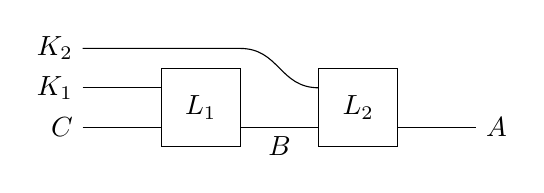
\begin{tikzpicture}[yscale=0.5]
    \draw (0,2) node[left] {$K_2$} -- (2,2) .. controls +(0.5,0) and +(-0.5,0) .. (3,1);
    \draw (0,1) node[left] {$K_1$} -- (1,1);
    \draw (0,0) node[left] {$C$} -- (1,0);
    \draw (2,0) -- node[below] {$B$} (3,0);
    \draw (4,0) -- (5,0) node[right] {$A$};
    \draw (1,1.5) rectangle node {$L_1$} (2,-0.5);
    \draw (3,1.5) rectangle node {$L_2$} (4,-0.5);
  \end{tikzpicture}
\]
Formally,
composition is defined as follows.

\begin{definition}[Composition] \label{def:slcomp}
Given two stateful components
$\Sigma_1 = (K_1 \mid L_1) : B \rightarrow C$ and
$\Sigma_2 = (K_2 \mid L_2) : A \rightarrow B$,
we define their composition
$\Sigma_1 \circ \Sigma_2 : A \rightarrow C$
in the following way:
\[
  \Sigma_1 \circ \Sigma_2 :=
    ( K_1 \times K_2 \mid L_1@K_2 \odot L_2 )
\]
Note that this formulation
implicitly uses the isomorphism
\[
  L_1@K_2 : B@K_2 \twoheadrightarrow (C@K_1)@K_2 \cong C@(K_1 \times K_2)
  \,.
\]
\end{definition}




\begin{lemma}
  This is compatible with:
  \begin{itemize}
    \item simple simulations;
    \item lifting hence associativity is preserved.
  \end{itemize}

\end{lemma}

%}}}

\subsection{Combining Hidden and Explicit State} %{{{

It is possible for a stateful component
to hide only part of the explicit state
used by the underlying transition system.
For example,
in a transition system
$L : A \rightarrow B@(K \times U) \cong B@U@K$,
we may choose to hide only $K$,
to obtain a stateful component
$\Sigma = (K \mid L) : A \rightarrow B@U$
which still exchanges explicit state of type $U$
with the environment.
This makes it possible to construct
complex stateful components incrementally
from simpler, stateless parts,
by first promoting them using $\&$,
then hiding state in a step-by-step fashion
using $\kw{fbk}$.

In addition,
stateful components can be lifted
to pass through explicit state.

\begin{definition} \label{def:slift}
The stateful component $\Sigma = (K \mid L) : A \rightarrow B$
can be lifted to \[ \Sigma@U := (K \mid L@U) : A@U \rightarrow B@U \,. \]
Note that this relies on the isomorphism
\[
  L@U : A@U \twoheadrightarrow (B@K)@U \cong (B@U)@K
  \,.
\]
\end{definition}

The following properties
relate the promotion operator $\&$,
the composition operators $\odot$ and $\circ$,
and the hiding operator $\kw{fbk}$.

\begin{lemma}
  For $L_1 : B \twoheadrightarrow C@K_1$ and
  $L_2 : A \twoheadrightarrow B@K_2$,
  the following property holds:
  \[
    \&L_1 \circ \&L_2 \equiv \&(L_1 \odot L_2)
    \,.
  \]
  In addition, for $\Sigma_1 : B \rightarrow C@U_1$
  and $\Sigma_2 : A \rightarrow B@U_2$,
  the following property holds:
  \[
    \kw{fbk}_{U_1}(\Sigma_1) \circ \kw{fbk}_{U_2}(\Sigma_2) \equiv
    \kw{fbk}_{U_1 \times U_2}(\Sigma_1@U_2 \circ \Sigma_2)
    \,.
  \]
\end{lemma}

%}}}

\subsection{Stateful Simulations} %{{{

Definition~\ref{def:ssim} introduced a simple notion of refinement
between stateful components,
but assumed that the interactions of both components
with their environment were identical.
By contrast, a key feature of CompCertO
is the notion of \emph{simulation convention},
which parameterizes simulations by
specifying how the interactions of
the source-level and target-level transition system
are related.

\subsubsection{Stateful Simulation Conventions} %{{{

Transition systems in CompCertO are stateless,
and as a consequence,
successive activations of given
source- and target-level
transition systems can be related in the same way.
By contrast,
our components may maintain encapsulated states
and behave differently upon successive activations.
As a consequence,
the relationship between source- and target-level interactions
may depend on the history of the computation.
This means we must generalize simulation conventions
so that they may maintain their own state as well.

\begin{definition} \label{def:sconv} %{{{
A \emph{stateful simulation convention}
$\mathbf{R} = \langle W, {\leadsto}, {\mapsto}, R^\que, R^\ans \rangle$
between the language interfaces $A^\sharp$ and $A^\flat$
is specified by:
\begin{itemize}
  \item a pointed set of worlds $W$,
    which store the current state of the simulation convention;
  \item two accessibility relations
    ${\leadsto}, {\mapsto} \subseteq W \times W$,
    corresponding to \emph{internal} and \emph{external} transitions;
  \item a Kripke relation $R^\que \in \mathcal{R}_W(A_\sharp^\que, A_\flat^\que)$
    between the language interfaces' questions, and
  \item a Kripke relation $R^\ans \in \mathcal{R}_W(A_\sharp^\ans, B_\flat^\ans)$
    between their answers.
\end{itemize}
The accessibility relations are required to be reflexive and transitive.
We write $\mathbf{R} : A^\sharp \leftrightarrow A^\flat$.
The identity simulation convention
$\kw{id}_A : A \leftrightarrow A$
is given by
$\kw{id}_A := \langle
    \mathbbm{1}, {=}_\mathbbm{1}, {=}_\mathbbm{1}, {=}_{A^\que}, {=}_{A^\ans}
 \rangle$.
\end{definition}
%}}}

The initial world $\intl{w}$ gives the simulation convention's initial state.
While the environment is in control,
the world may transition according to the relation $\mapsto$.
When control is transferred to the system,
the corresponding questions must be related by $w \Vdash R^\que$.
World transitions may then occur according to $\leadsto$.
Hence, when the system returns control to the environment,
the corresponding answers
will be related by $w' \Vdash R^\ans$,
where $w'$ is a successor world of $w$ such that $w \leadsto w'$.
The questions for any subsequent activation
must in turn be related at a world $w''$ such that $w' \mapsto w''$,
and so on and so forth indefinitely:
\begin{align*}
  \intl{w} \mapsto w_1 &\Vdash q^\sharp_1 \mathrel{R^\que} q^\flat_1 \\
  w_1 \leadsto w_1' &\Vdash r^\sharp_1 \mathrel{R^\ans} r^\flat_1 \\
  w_1' \mapsto w_2 &\Vdash q^\sharp_2 \mathrel{R^\que} q^\flat_2 \\
  w_2 \leadsto w_2' &\Vdash r^\sharp_2 \mathrel{R^\ans} r^\flat_2 \\[-1ex]
  &\:\:\vdots
\end{align*}

%}}}

\subsubsection{Stateful Simulations of Transition Systems} %{{{

Before we define simulations between stateful components,
we first update CompCertO's notion of simulation of transition systems
to take into account stateful conventions.
%In particular,
%using stateful simulation conventions,
%the sequence of external calls performed by a transition system
%will become important.

Consider a simulation of type:
\[
\begin{tikzcd}
  A_1 \ar[r, twoheadrightarrow, "L_1"] \ar[d, leftrightarrow, "\mathbf{R}_A"'] &
  B_1 \ar[d, leftrightarrow, "\mathbf{R}_B"] \\
  A_2 \ar[r, twoheadrightarrow, "L_2"] & B_2
\end{tikzcd}
\]
The simulation simultaneously
plays the role of the system with respect to
the simulation convention $\mathbf{R}_B$ and
the role of the environment with respect to $\mathbf{R}_A$.
Hence,
it will operate in the context of a Kripke frame
constructed from both $W_A$ and $W_B$.
The possible states of a simulation will be a subset
$W \subseteq W_A \times W_B$,
which must contain
the initial state $\intl{w} := (\intl{w}_A, \intl{w}_B) \in W$.
Between successive activations,
the environment may update the $W_B$ component.
Hence we require:
\[
  (w_A, w_B) \in W \:\wedge\:
  w_B \mapsto_B w_B' \:\Rightarrow\:
  (w_A, w_B') \in W
\]
When the components execute,
the worlds will evolve according to
the accessibility relation:
\[
  (w_A, w_B) \leadsto_{\bar{A}B} (w_A', w_B') \::\Leftrightarrow\:
  w_A \mapsto_A w_A' \:\wedge\: w_B \leadsto_B w_B'
\]
Reading the constituent transition relations
within $L_1, L_2$ as functions of type:
\begin{align*}
  I_1 &: B_1^\que \rightarrow \mathcal{P}(S_1) &
  {\rightarrow_1} &: S_1 \rightarrow \mathcal{P}(\mathbb{E}^* \times S_1) &
  F_1 &: S_1 \rightarrow \mathcal{P}(B_1^\ans)
  \\
  I_2 &: B_2^\que \rightarrow \mathcal{P}(S_2) &
  {\rightarrow_2} &: S_2 \rightarrow \mathcal{P}(\mathbb{E}^* \times S_2) &
  F_2 &: S_2 \rightarrow \mathcal{P}(B_2^\ans)
  \,,
\end{align*}
we can formulate the simulation properties for internal steps
concisely as shown in Fig.~\ref{fig:simint}.
\begin{figure}[h]
  \small
  \[
    \begin{array}{c@{\qquad}c@{\qquad}c}
      \begin{tikzcd}[sep=tiny,column sep=0]
        q_1 \ar[dd, "w \Vdash \mathbb{R}_B^\que"', dash] \ar[rr, dash, "I_1"] &&
        s_1 \ar[dd, "w' \Vdash R", dash, dashed] \\
        & \leadsto_{\bar{A}B} & \\
        q_2 \ar[rr, "I_2"', dash, dashed] &&
        s_2
      \end{tikzcd}
      &
      \begin{tikzcd}[sep=tiny,column sep=0]
        s_1 \ar[rr, "t"] \ar[dd, "w \Vdash R"', dash] &&
        \!\!{}_1 \:\, s_1' \ar[dd, "w' \Vdash R", dash, dashed] \\
        & \leadsto_{\bar{A}B} & \\
        s_2 \ar[rr, "t", dashed] &&
        \!\!{}_2^* \:\, s_2'
      \end{tikzcd}
%      \begin{tikzcd}[sep=large]
%        s_1 \ar[r] \ar[d, "{(w_A, w_B) \Vdash R}"', dash] &
%        s_1' \ar[d, "{(w_A,w_B) \Vdash R}", dash, dashed] \\
%        s_2 \ar[r, dashed] &
%        \!\!\!{}^* \: s_2'
%      \end{tikzcd}
      &
      \begin{tikzcd}[sep=tiny, column sep=0]
        s_1 \ar[rr, "F_1", dash] \ar[dd, "w \Vdash R"', dash] &&
        r_1 \ar[dd, "w' \Vdash \mathbb{R}_B^\ans", dash, dashed] \\
        & \leadsto_{\bar{A}B} & \\
        s_2 \ar[rr, "F_2"', dash, dashed] &&
        r_2
      \end{tikzcd}
      \vspace{1ex} \\
      I_1 \ifr{\Vdash \mathbb{R}_B^\que \rightarrow
        \mathcal{P}^\le(\Diamond_{\bar{A}B} R)} I_2
      &
      {\rightarrow_1}
      \ifr{\Vdash R \rightarrow \mathcal{P}^\le(\Diamond_{\bar{A}B} ({=} \times R))}
      {\rightarrow_2^*}
      &
      F_1
      \ifr{\Vdash R \rightarrow \mathcal{P}^\le(\Diamond_{\bar{A}B} \mathbb{R}_B^\ans)}
      F_2
      \vspace{1.2ex} \\
      \text{(a) Initial states} &
      \text{(b) Internal states} &
      \text{(c) Final states}
    \end{array}
  \]
  \caption{Stateful simulation properties for internal steps}
  \label{fig:simint}
\end{figure}

Conversely, for external calls,
the simulation plays the role of the environment.
We expect that:
\[
  (w_A, w_B) \in W \:\wedge\:
  w_A \leadsto_A w_A' \:\Rightarrow\:
  (w_A', w_B) \in W
\]
Moreover,
from the point of view of the simulation,
an external call will make a transition according to
the following accessibility relation:
%[NB we may want to restrict $\leadsto_B$ to $=$
%if this causes problems, but]
%Note that by allowing a transition $w_B \leadsto_B w_B'$,
%we are able to capture the effect that
%any reentrant call may have on the simulation state:
\[
  (w_A, w_B) \leadsto_{AB} (w_A', w_B') \::\Leftrightarrow\:
  w_A \leadsto_A w_A' \:\wedge\:
  w_B = w_B'
\]
By reading the action of transition systems at external calls
in terms of the functions:
\begin{align*}
  Z_1 &: S_1 \rightarrow
    \mathcal{P}(A_1^\que \times (A_1^\ans \rightarrow \mathcal{P}(S_1))) &
  Z_1(s_1) &:= \{ (q_1, Y_1^{s_1}) \mid s_1 \mathrel{X_1} q_1 \}
 \\
  Z_2 &: S_2 \rightarrow
    \mathcal{P}(A_2^\que \times (A_2^\ans \rightarrow \mathcal{P}(S_2))) &
  Z_2(s_2) &:= \{ (q_2, Y_2^{s_2}) \mid s_2 \mathrel{X_2} q_2 \}
  \,,
\end{align*}
we can then formulate the simulation condition for external calls
as presented in Fig.~\ref{fig:simext} below.

\begin{figure}[h]
  \[
    \begin{array}{c}
      \begin{tikzcd}[sep=tiny, column sep=small]
        s_1 \ar[rr, "X_1", dash] \ar[dd, "w \Vdash R"', dash] &&
        m_1 \ar[rr, dotted, dash] \ar[dd, "w'"', "{} \Vdash \mathbb{R}_A^\que", dash, dashed] &&
        n_1 \ar[rr, "Y_1^{s_1}", dash] \ar[dd, "w''"', "{} \Vdash \mathbb{R}_A^\ans", dash] &&
        s_1' \ar[dd, "w''' \Vdash R", dash, dashed]
        \\
        & \leadsto_{\bar{A}B} && \leadsto_{AB} && \leadsto_{\bar{A}B} &
        \\
        s_2 \ar[rr, "X_2"', dash, dashed] &&
        m_2 \ar[rr, dotted, dash] &&
        n_2 \ar[rr, "Y_2^{s_2}"', dash, dashed] &&
        s_2'
      \end{tikzcd}
      \vspace{1ex} \\
      Z_1
      \mathrel{[
        \Vdash R \rightarrow \mathcal{P}^\le(
          \Diamond_{\bar{A}B} (
          \mathbb{R}_A^\que \times
            \Box_{AB} (
            \mathbb{R}_A^\ans \rightarrow
            \mathcal{P}^\le(\Diamond_{\bar{A}B} R))))
      ]}
      Z_2
    \end{array}
  \]
  \caption{Simulation property for external states}
  \label{fig:simext}
\end{figure}

\begin{definition}[Stateful simulation]
A stateful simulation of CompCertO transition systems,
written as
$L_1 \preceq_{\mathbb{R}_A \twoheadrightarrow \mathbb{R}_B} L_2$,
is given by a set of worlds $W$ such that
\[ (\intl{w}_A, \intl{w}_B) \in W \subseteq W_A \times W_B \,, \]
closed under ${\leadsto_A} \times {\mapsto_B}$,
satisfying the properties given in
\autoref{fig:simint} and
\autoref{fig:simext}.
\end{definition}

Note that the stateless simulation conventions of CompCertO
can be promoted as follows.

\begin{definition}[Promoted simulation convention]
The CompCertO simulation convention
$\mathbb{R} = \langle W, \mathbb{R}^\que, \mathbb{R}^\ans \rangle$
can be promoted to the stateful simulation convention
$\&\mathbb{R} :=
 \langle W_*, {=}, \top, \mathbb{R}^\que_*, \mathbb{R}^\ans_* \rangle$.
The pointed set $W_* = W \cup \{ \intl{*} \}$
introduces a new initial world $*$.
The relations $\mathbb{R}^\que_*$ and $\mathbb{R}^\ans_*$
are empty at this initial world,
but the environment can transition
to any world $w \in W$ (${\mapsto} := \top$).
The system must leave the world unchanged (${\leadsto} := {=}$).
\end{definition}

Then we have the relationship:
\begin{lemma}[CompCertO \emph{vs\@.} stateful simulations]
\[
  L_1 \le_{\mathbb{R}_A \twoheadrightarrow \mathbb{R}_B} L_2
  \quad \Leftrightarrow \quad
  L_1 \preceq_{\&\mathbb{R}_A \twoheadrightarrow \&\mathbb{R}_B} L_2
\]
\end{lemma}

As with simulations in CompCertO,
stateful simulations compose both horizontally and vertically.
The horizontal (layered) composition of simulations
is as follows.

\begin{lemma}[Layered composition of stateful simulations]
\[
  \begin{prooftree}
    \hypo{
      L_1^\sharp
      \preceq_{\mathbf{R}_B \twoheadrightarrow \mathbf{R}_C}
      L_1^\flat}
    \hypo{
      L_2^\sharp
      \preceq_{\mathbf{R}_A \twoheadrightarrow \mathbf{R}_B}
      L_2^\flat}
    \infer2{
      L_1^\sharp \odot L_2^\sharp
      \preceq_{\mathbf{R}_A \twoheadrightarrow \mathbf{R}_C}
      L_1^\flat \odot L_2^\flat}
  \end{prooftree}
  \qquad \qquad
  \begin{tikzcd}
    A^\sharp \ar[r, twoheadrightarrow, "L_2^\sharp"]
	     \ar[d, leftrightarrow, "\mathbf{R}_A"] &
    B^\sharp \ar[r, twoheadrightarrow, "L_1^\sharp"]
	     \ar[d, leftrightarrow, "\mathbf{R}_B"] &
    C^\sharp \ar[d, leftrightarrow, "\mathbf{R}_C"]
    \\
    A^\flat \ar[r, twoheadrightarrow, "L_2^\flat"'] &
    B^\flat \ar[r, twoheadrightarrow, "L_1^\flat"'] &
    C^\flat
  \end{tikzcd}
\]
\end{lemma}

To formulate vertical composition, we must first explain how
the stateful simulation conventions themselves compose.

\begin{definition}[Composition of Stateful Conventions] \label{def:sccomp}
Given the stateful simulation conventions
$\mathbf{R}_1 : A^\sharp \leftrightarrow A^\natural$ and
$\mathbf{R}_2 : A^\natural \leftrightarrow A^\flat$,
the composite simulation convention
$\mathbf{R}_1 \mathbin; \mathbf{R}_2 : A^\sharp \leftrightarrow A^\flat$
has the following components:
\begin{gather*}
  W := W_1 \times W_2 \\
  (w_1, w_2) \mapsto (w_1', w_2') \: :\Leftrightarrow \:
    w_1 \mapsto_1 w_1' \: \wedge \:
    w_2 \mapsto_2 w_2' \\
  (w_1, w_2) \leadsto (w_1', w_2') \: :\Leftrightarrow \:
    w_1 \leadsto_1 w_1' \: \wedge \:
    w_2 \leadsto_2 w_2' \\
  R^\que := R_1^\que \cdot R_2^\que \\
  R^\ans := R_1^\ans \cdot R_2^\ans
\end{gather*}
\end{definition}

\begin{lemma}
$ \&(\mathbb{R}_1 \cdot \mathbb{R}_2) \equiv
   \&\mathbb{R}_1 \mathop; \&\mathbb{R}_2 $
\quad
[But we need to define simulation convention refinement]
\end{lemma}

\begin{theorem}[Vertical composition of stateful simulations] %\label{thm:svcomp}
\[
  \begin{prooftree}
    \hypo{L^\sharp
      \preceq_{\mathbf{R}_A \twoheadrightarrow \mathbf{R}_B}
      L^\natural}
    \hypo{L^\natural
      \preceq_{\mathbf{S}_A \twoheadrightarrow \mathbf{S}_B}
      L^\flat}
    \infer2{L^\sharp
      \preceq_{\mathbf{R}_A \mathbin; \mathbf{S}_A \twoheadrightarrow
	   \mathbf{R}_B \mathbin; \mathbf{S}_B}
      L^\flat}
  \end{prooftree}
\]
\end{theorem}

%}}}

%}}}

\subsection{Simulation of Stateful Components} %{{{

We have defined stateful simulations of transition systems.
We now seek to extend them to cover stateful components.
Such simulations will essentially be
stateful simulations between the underlying transition systems.
However,
because encapsulated states are not observed by the environment,
we expect a simulation between the stateful components
$\Sigma^\sharp : A^\sharp \rightarrow B^\sharp$ and
$\Sigma^\flat : A^\flat \rightarrow B^\flat$
to be typed as
$
  \Sigma^\sharp \preceq_{\mathbf{R}_A \rightarrow \mathbf{R}_B}
  \Sigma^\flat
$
with $\mathbf{R}_B : B^\sharp \leftrightarrow B^\flat$.
The challenge is then to make it possible for
the internal states of the underlying transition systems
$L^\sharp : A^\sharp \rightarrow B^\sharp@K^\sharp$
and
$L^\flat : A^\flat \rightarrow B^\flat@K^\flat$
to be taken into account by the simulation.

Our solution will be to construct a simulation convention
$\mathbf{R}_B@\langle K^\sharp, K^\flat \rangle :
 B^\sharp@K^\sharp \leftrightarrow B^\flat@K^\flat$,
which will incorporate states into the worlds
but otherwise behave identically to $\mathbf{R}_B$.

\begin{definition}[Lifting simulation conventions] \label{def:liftsconv} %{{{
For a stateful convention
$\mathbf{R} : A^\sharp \leftrightarrow A^\flat$
and two pointed sets $K^\sharp, K^\flat$, 
we define %the stateful convention
$\mathbf{R}@\langle K^\sharp,K^\flat \rangle :
   A^\sharp@K^\sharp \leftrightarrow A^\flat@K^\flat$
with the following components:
\begin{gather*}
  W := W_\mathbf{R} \times K^\sharp \times K^\flat
  \qquad
  \intl{w} := \big( \intl{w}_\mathbf{R}, \intl{k}^\sharp, \intl{k}^\flat \big)
  \\
 {\begin{prooftree}
    \hypo{w \leadsto_\mathbf{R} w'}
    \infer1{(w, k_\sharp, k_\flat) \leadsto (w', k_\sharp', k_\flat')}
  \end{prooftree}}
  \qquad
 {\begin{prooftree}
    \hypo{w \mapsto_\mathbf{R} w'}
    \infer1{(w, k^\sharp, k^\flat) \mapsto (w', k^\sharp, k^\flat)}
  \end{prooftree}}
  \\
 {\begin{prooftree}
    \hypo{w \Vdash q^\sharp \mathrel{\mathbf{R}^\que}
                   q^\flat}
    \infer1{
      (w, k^\sharp, k^\flat) \Vdash
      q^\sharp@k^\sharp
      \mathrel{[\mathbf{R}@\langle K_1, K_2 \rangle]^\que}
      q^\flat@k^\flat}
  \end{prooftree}}
  \qquad
 {\begin{prooftree}
    \hypo{w \Vdash r^\sharp \mathrel{\mathbf{R}^\ans}
                   r^\flat}
    \infer1{
      (w, k^\sharp, k^\flat) \Vdash
      r^\sharp@k^\sharp
      \mathrel{[\mathbf{R}@\langle K_1, K_2 \rangle]^\ans}
      r^\flat@k^\flat}
  \end{prooftree}}
\end{gather*}
\end{definition}
%}}}

For simulations of stateful components,
the underlying simulation of transition systems
can then operate in terms
of the instrumented simulation convention defined above.
In particular, this allows
the (existentially quantified) world invariant
$W \subseteq W_A \times W_B \times K^\sharp \times K^\flat$
used by the simulation
to impose constraints on the encapsulated states.

\begin{definition}[Simulation] \label{def:ssim} %{{{
There is a \emph{simulation} of type
\[
  \Sigma^\sharp \preceq_{\mathbf{R}_A \rightarrow \mathbf{R}_B} \Sigma^\flat
  \qquad \qquad
\begin{tikzcd}
  A^\sharp \ar[r, "\Sigma^\sharp"]
      \ar[d, leftrightarrow, "\mathbf{R}_A"'] &
  B^\sharp \ar[d, leftrightarrow, "\mathbf{R}_B"] \\
  A^\flat \ar[r, "\Sigma^\flat"] &
  B^\flat
\end{tikzcd}
\]
between
the stateful components
$\Sigma^\sharp = (K^\sharp \mid L^\sharp) : A^\sharp \rightarrow B^\sharp$ and
$\Sigma^\flat = (K^\flat \mid L^\flat) : A^\flat \rightarrow B^\flat$
when
\[
  L^\sharp
  \preceq_{\mathbf{R}_A \rightarrow
           \mathbf{R}_B@\langle K^\sharp, K^\flat \rangle}
  L^\flat
  \,.
\]
\end{definition}
%}}}

Defined in this way,
simulations of stateful components generalize
the original simulations used in CompCertO.
First,
basic simulations between transition systems
can be promoted to stateful simulations.
Then,
these stateful simulations induce
simulations between the corresponding
embedded stateful components.

\begin{lemma}[Promoting simulations] %{{{
\[
  \begin{prooftree}
    \hypo{L^\sharp
      \le_{\mathbb{R}_A \twoheadrightarrow \mathbb{R}_B}
      L^\flat}
    \infer1{L^\sharp
      \preceq_{\&\mathbb{R}_A \twoheadrightarrow \&\mathbb{R}_B}
      L^\flat}
  \end{prooftree}
  \qquad
  \begin{prooftree}
    \hypo{L^\sharp
      \preceq_{\mathbf{R}_A \twoheadrightarrow \mathbf{R}_B}
      L^\flat}
    \infer1{\&L^\sharp
      \preceq_{\mathbb{R}_A \rightarrow \mathbb{R}_B}
      \&L^\flat}
  \end{prooftree}
\]
\end{lemma}
%}}}

Moreover,
simulations of stateful components satisfy the expected
composition properties.

\begin{lemma}[Layered composition of simulations] \label{thm:slcompsim} %{{{
\[
  \begin{prooftree}
    \hypo{
      \Sigma_1^\sharp
      \preceq_{\mathbf{R}_B \rightarrow \mathbf{R}_C}
      \Sigma_1^\flat}
    \hypo{
      \Sigma_2^\sharp
      \preceq_{\mathbf{R}_A \rightarrow \mathbf{R}_B}
      \Sigma_2^\flat}
    \infer2{
      \Sigma_1^\sharp \circ \Sigma_2^\sharp
      \preceq_{\mathbf{R}_A \rightarrow \mathbf{R}_C}
      \Sigma_1^\flat \circ \Sigma_2^\flat}
  \end{prooftree}
  \qquad
  \begin{tikzcd}
    A^\sharp \ar[r, rightarrow, "\Sigma_2^\sharp"]
	     \ar[d, leftrightarrow, "\mathbf{R}_A"] &
    B^\sharp \ar[r, rightarrow, "\Sigma_1^\sharp"]
	     \ar[d, leftrightarrow, "\mathbf{R}_B"] &
    C^\sharp \ar[d, leftrightarrow, "\mathbf{R}_C"]
    \\
    A^\flat \ar[r, rightarrow, "\Sigma_2^\flat"'] &
    B^\flat \ar[r, rightarrow, "\Sigma_1^\flat"'] &
    C^\flat
  \end{tikzcd}
\]
\end{lemma}
%}}}

\begin{lemma}[Vertical composition of simulations] \label{thm:svcomp} %{{{
\[
  \begin{prooftree}
    \hypo{\Sigma^\sharp
      \preceq_{\mathbf{R}_A \twoheadrightarrow \mathbf{R}_B}
      \Sigma^\natural}
    \hypo{\Sigma^\natural
      \preceq_{\mathbf{S}_A \twoheadrightarrow \mathbf{S}_B}
      \Sigma^\flat}
    \infer2{\Sigma^\sharp
      \preceq_{\mathbf{R}_A \mathbin; \mathbf{S}_A \twoheadrightarrow
	   \mathbf{R}_B \mathbin; \mathbf{S}_B}
      \Sigma^\flat}
  \end{prooftree}
\]
\end{lemma}
%}}}

[This means in particular that language interfaces and stateful components
also constitute a double category,
and our embedding constitutes a double functor.]

%}}}

\subsection{Relating Hidden and Explicit State} %{{{

To conclude this section we discuss how
state encapsulation primitives and simulations interact.

Recall that in Definition~\ref{def:liftsconv}, we defined a simulation convention
$\mathbf{R}@\langle K^\sharp, K^\flat \rangle$,
which was then used in Definition~\ref{def:ssim}
to relate the underlying transition systems
of stateful components.
Expressed in the context of the state encapsulation primitive $\kw{fbk}$,
this gives rise to the following principle.

\begin{lemma}[Proving simulations for encapsulated components] \label{thm:fbksim}
\[
  \begin{prooftree}
    \hypo{\Sigma^\sharp
      \preceq_{\mathbf{R}_A \rightarrow
	       \mathbf{R}_B@\langle K^\sharp,K^\flat \rangle}
      \Sigma^\flat}
    \infer1{\kw{fbk}_{K^\sharp}(\Sigma^\sharp)
      \preceq_{\mathbf{R}_A \rightarrow \mathbf{R}_B}
      \kw{fbk}_{K^\flat}(\Sigma^\flat)}
  \end{prooftree}
\]
\end{lemma}

Because of the properties of $\kw{fbk}$,
and because state can be hidden incrementally,
the source and target transition systems in a simulation
may differ in how much of their state is encapsulated.
For example,
we will often want to show that
a given high-level component with encapsulated state
is realized by a low-level implementation
where all state remains explicit.
In this case,
the stateful convention used by the simulation
will enforce the expectation that
the context may not modify the concrete explicit state
between successive invocations of the component.

In the simplest case,
suppose we want to show a simulation between the stateful component
$\kw{fbk}_K(\Sigma) : A \rightarrow B$ which encapsulates $K$
and the ``naked'' underlying component $\Sigma : A \rightarrow B@K$.
We must choose a simulation convention
$\kw{reveal}_{B,K} : B \leftrightarrow B@K$ such that
$
  \Sigma
  \preceq_{\kw{id}_A \rightarrow \kw{reveal}_{B,K}@\langle K, \mathbbm{1} \rangle}
  \Sigma
$.
Since $\Sigma \equiv \kw{fbk}_\mathbbm{1}(\Sigma)$,
we can then apply Theorem~\ref{thm:fbksim} to obtain
the desired simulation property
\[
  \kw{fbk}_K(\Sigma)
  \preceq_{\kw{id}_A \rightarrow \kw{reveal}_{B,K}}
  \Sigma
  \,.
\]
Such a simulation convention can in fact be defined in the general case.

\begin{definition}
For a simulation convention
$\mathbf{R} : A^\sharp@K^\sharp \leftrightarrow A^\flat@K^\flat$,
we define the simulation convention
$\kw{fbk}_{K^\sharp,K^\flat}(\mathbf{R}) :
 A^\sharp \leftrightarrow A^\flat$
as follows:
\begin{gather*}
  W := W_\mathbf{R} \times K^\sharp \times K^\flat
  \qquad \intl{w} := (\intl{w}_\mathbf{R}, \intl{k}^\sharp, \intl{k}^\flat)
  \\[1ex]
 {\begin{prooftree}
    \hypo{w \leadsto_\mathbf{R} w'}
    \infer1{(w, k_\sharp, k_\flat) \leadsto (w', k_\sharp', k_\flat')}
  \end{prooftree}}
  \qquad
 {\begin{prooftree}
    \hypo{w \mapsto_\mathbf{R} w'}
    \infer1{(w, k^\sharp, k^\flat) \mapsto (w', k^\sharp, k^\flat)}
  \end{prooftree}}
  \\[1ex]
 {\begin{prooftree}
    \hypo{w \Vdash q^\sharp@k^\sharp \mathrel{\mathbf{R}^\que}
                   q^\flat@k^\flat}
    \infer1{
      (w, k^\sharp, k^\flat) \Vdash
      q^\sharp
      \mathrel{[\kw{fbk}_{K^\sharp,K^\flat}(\mathbf{R})]^\que}
      q^\flat}
  \end{prooftree}}
  \qquad
 {\begin{prooftree}
    \hypo{w \Vdash r^\sharp@k^\sharp \mathrel{\mathbf{R}^\ans}
                   r^\flat@k^\flat}
    \infer1{
      (w, k^\sharp, k^\flat) \Vdash
      r^\sharp
      \mathrel{[\kw{fbk}_{K^\sharp,K^\flat}(\mathbf{R})]^\ans}
      r^\flat}
  \end{prooftree}}
\end{gather*}
\end{definition}

\begin{lemma}[XXX: Somewhat speculative]
\[
  \mathbf{R}
  \:\sqsubseteq\:
  \kw{fbk}_{K^\sharp,K^\flat}(\mathbf{R})@\langle K^\sharp, K^\flat \rangle
\]
\end{lemma}

%$\kw{fbk}_{K_1,K_2}(\mathbb{R}@R_K) \sqsubseteq \mathbb{R}$
%\begin{proof}
%We would have to define refinement for stateful simulation conventions
%for this question to even make sense to begin with.
%\end{proof}

Combined with Theorem~\ref{thm:fbksim},
this entails the following property.

\begin{lemma}
\[
  \begin{prooftree}
    \hypo{\Sigma_1 \preceq_{\mathbb{R}_A \rightarrow \mathbb{R}_B} \Sigma_2}
    \infer1{
      \kw{fbk}_{K_1}(\Sigma_1)
      \preceq_{\mathbb{R}_A \rightarrow \kw{fbk}_{K_1, K_2}(\mathbb{R}_B)}
      \kw{fbk}_{K_2}(\Sigma_2)}
  \end{prooftree}
\]
\end{lemma}

We can the define the simulation convention $\kw{reveal}_{B,K}$ as:
\[
  \kw{reveal}_{B,K} := \kw{fbk}_{K,\mathbbm{1}}(\kw{id}_{B@K}) : B \leftrightarrow B@K
  \,,
\]
such that in particular:
\[
  \kw{fbk}_K(\Sigma)
  \preceq_{A \rightarrow \kw{reveal}_K(B)}
  \Sigma
  \,.
\]

%}}}

%}}}

\section{Clight with module-local state} %{{{

[Note: this could be swapped with Section 3
because it showcases the use of persistent state,
but probably does not have much to gain
from the memory separation framework.]

Can we add a $\mathsf{private}$ keyword or storage class to Clight,
formulate a semantics and show a correctness proof
for erasure of the keyword?

Main challenge: how to define the semantics of the new keyword
in a way that's convenient.

We need a good name for this language.
For now I will use \ClightP{}.

\subsection{Syntax}

\ClightP{} programs are identical to Clight programs,
but allow the definition of module-local, private variables.
For example:

\begin{minted}{C}
private int c = 0;
int count(void) { return c++; }
\end{minted}

One question is whether such private variables
should be declared as globals
(perhaps associated with empty memory blocks)
or if we should have a custom \mintinline{Coq}{program} type.

\subsection{Semantics}

Private variables in a \ClightP{} program
are not stored in the memory,
but rather in a separate environment.
This environment is similar to
the local environments used to store temporaries
(it might be possible to reuse the same type),
but instead of being used in the context of an activation,
the private environment is used as persistent state.
Hence for a program $p$, the \ClightP{} semantics is constructed
first by defining a transition system of type
\[
  L : \mathcal{C}@\mathsf{mem} \twoheadrightarrow
      \mathcal{C}@(\mathsf{mem}\times\mathsf{penv})
\]
and then hiding the private environment as persistent state:
\[
  \ClightP{}(p) := \mathsf{fbk}_\mathsf{penv}(\&L) :
    \mathcal{C}@\mathsf{mem} \rightarrow
    \mathcal{C}@\mathsf{mem}
\]

One subtlety in the case where private variables are globals,
is that the \texttt{initial\_state} predicate of $L$
must enforce empty permissions for private variables
in the incoming memory state.

\subsection{Compiling to Clight}

A \ClightP{} program can be compiled to Clight
by erasing the \texttt{private} annotations
and turning privates variable into regular
static variables.

Proving the correctness of this transformation
should not be too difficult.
We can just use a memory extension or injection.
The only new part is that we must express
the simulation convention for the underlying transition systems
in a way that relates the source private environment
to the target (public) memory state.
The twist here is that
the externally observable simulation convention
should just enforce the empty permissions in the source memory.
The relation between the private state and the target memory
should be existentially quantified.
But this means we need requirements on the initial target memory as well.
We will have to set up our extended notion of simulation
in a way that supports those things.

%}}}

\section{Memory Separation in CompCert} %{{{

\subsection{Status quo} %{{{

Explain how injections are used in CompCert, CompCertO, CAL,
and why it's too complex.
The \emph{algebraic memory model} used in CCAL
is closer to typical separation algebra
but there are issues with nextblock.
Fortunately Nominal CompCert allows us to
do better.

%}}}

\subsection{A separation algebra for CompCert memory} %{{{

The goal is to define a ternary relation:
\[
    m_1 \bullet m_2 \equiv m
\]
asserting that the memory states $m_1$ and $m_2$
can be merged into $m$.

We can proceed recursively by defining
relations of this kind incrementally on:
\begin{itemize}
  \item runtime values $\mathsf{val}$,
  \item memory permissions,
  \item whole memory states.
\end{itemize}

As in CCAL,
the challenge is to deal with nextblock.
This is where Nominal CompCert can help
by figuring out a way to partition the block space
between a component and its context.
Can the stack-aware version be helpful
by discriminating between blocks allocated
for each function?

%}}}

\begin{figure}
  \fbox{$\kw{option}\ \kw{perm} \times \kw{memval}$}
  \begin{gather*}
    (\bot, \kw{undef}) \bullet (p, v) \equiv (p, v) \\
    (p, v) \bullet (\bot, \kw{undef}) \equiv (p, v)
  \end{gather*}
\end{figure}

\subsection{Frame rule} %{{{

The properties listed in Fig.~X
compose and ultimately ensure that
more complex ways to manipulate memory states
remain compatible with the memory separation relation.
Ultimately this allows us to derive
a kind of \emph{frame rule} for the Clight semantics.
We can state this informally as follows:
\[
  \begin{prooftree}
    \hypo{\kw{Clight}(p) : m_1 \leadsto m_2}
    \infer1{\kw{Clight}(p) : m_1 \bullet m \leadsto m_2 \bullet m}
  \end{prooftree}
\]
In other words,
if the program $p$ safely acts on a memory state $m_1$
to transform it into a memory state $m_2$,
then we can frame a memory fragment $m$ onto $m_1$
and expect the program to leave that fragment intact.
Intuitively, this holds because
if $p$ ever needed or affected any of the memory present
in fragment $m$,
it would have gone wrong on $m_1$ alone.

To formalize this property in the context of CompCertO,
we can promote the memory separation relation
to a simulation convention:
\[
  \forall A \:.\quad
  A@{\bullet} : A@(\kw{mem} \times \kw{mem}) \Leftrightarrow A@\kw{mem}
\]
We will then compare the ``source''-level semantics
\[
  \kw{Clight}(p)@\kw{mem} :
    \mathcal{C}@(\kw{mem} \times \kw{mem}) \twoheadrightarrow
    \mathcal{C}@(\kw{mem} \times \kw{mem})
  \,,
\]
which acts on one of the memory fragments
but leaves the other one unchanged,
to the concrete semantics of $p$ acting on the total memory state:
\[
  \kw{Clight}(p) : \mathcal{C}@\kw{mem} \Leftrightarrow \mathcal{C}@\kw{mem}
  \,.
\]
This yields the following property.

\begin{lemma}[Frame rule for Clight]
\[
  \kw{Clight}(p)@\kw{mem}
  \le_{\mathcal{C}@{\bullet} \twoheadrightarrow \mathcal{C}@{\bullet}}
  \kw{Clight}(p)
\]
\end{lemma}

%}}}

\subsection{Hiding Memory State} %{{{

In \S\ref{sec:clightp:erasure}


%}}}

\subsection{Initial memory} %{{{

The way we define $\kw{init\_mem}$ can work with the
separation relation such that:
\[
  \kw{init\_mem}(p_1) \bullet \kw{init\_mem}(p_2) \equiv
  \kw{init\_mem}(p_1 + p_2)
\]

%}}}

\subsection{Implementing Memory Separation with Nominal CompCert} %{{{

%}}}

%}}}

\section{Certified Abstraction Layers} \label{sec:cal} %{{{

A cleaner version of our OOPSLA story.
Here we must go from:
\begin{itemize}
  \item A fully abstract version where the layer interface
    has encapsulated abstract state,
    but does not change the memory at all
  \item A version where this is realized by an encapsulated
    memory component,
    which is added when the layer is invoked,
    and re-separated when it returns control to the client
    (refinement can act on that individual memory fragment).
  \item The concrete implementation version
    where the state is part of the global memory
    (refinement shown via
    simulation up to ${-} \bullet m \equiv {-}$).
\end{itemize}

\subsection{Layer Interfaces} %{{{

A layer interface with abstract states in $D$
can be defined using a transition system:
\[
  L : \mathbf{1} \twoheadrightarrow \mathcal{C}@D
\]
To interface with context code,
we can hide the abstract state and lift the component to:
\[
  \kw{fbk}_D(\&L)@\kw{mem} : \mathbf{1} \rightarrow \mathcal{C}@\kw{mem}
\]
Note that the component above never modifies the global memory state.

%}}}

\subsection{Layer Implementation} %{{{

The correctness property $L^\flat \vdash M : L^\sharp$
must be established as a simulation of the form:
\[
  \kw{fbk}(\&L^\sharp)@\kw{mem}
  \le_\mathbb{R}
  \&\kw{Clight}(M) \circ \kw{fbk}(\&L^\flat)@\kw{mem}
  :
  \mathbf{1} \rightarrow \mathcal{C}@\kw{mem}
\]
Here the simulation convention $\mathbb{R}$
must exclude from the source memory
the region used in the target memory
to store the persistent state and stack frames used by $M$.
It must also ensure that
this region remains unchanged in the target memory
between successive activations of $M$.
However,
the exact representation used
to represent the hidden abstract state of $L^\sharp$
is itself hidden within the simulation.

\paragraph{Layer Correctness}

To prove a particular layer implementation correct,
we first focus on the way $M$ acts on its private fragment.
We give an abstraction relation
$R \subseteq D^\sharp \times (D^\flat \times \kw{mem})$
such that:
\begin{equation}
  L^\sharp
  \:\le_{\mathbf{1} \rightarrow \kw{id}@R}\:
  \kw{Clight}(M)@D^\flat \circ L^\flat@\kw{mem}
  \qquad \text{and} \qquad
  \intl{d}^\sharp \mathrel{R} \big( \intl{d}^{\,\flat}, \intl{m} \big)
  \,.
  \label{eqn:lc}
\end{equation}
Here $\intl{m}$ is the initial memory fragment for the module $M$,
derived from the definitions within $M$ itself.
Note that we can carry out this proof without regard for the context memory.
There are no particular conditions on $R$ other than
initial state being related.

\paragraph{Adding Context Memory}

By hiding internal state,
\autoref{eqn:lc} can be used to establish:
\begin{align*}
  \kw{fbk}_{D^\sharp}(\&L^\sharp) \le {} &
  \kw{fbk}_{D^\flat \times \kw{mem}} \big(
    \&(\kw{Clight}(M)@D^\flat \circ L^\flat@\kw{mem})
    \big) \\ \equiv {} &
  \kw{fbk}_\kw{mem}(\&\kw{Clight}(M)) \circ \kw{fbk}_{D^\flat}(\&L^\flat)
  : \mathbf{1} \rightarrow \mathcal{C}
  \,,
\end{align*}
however this does not take into account the context memory,
or the way in which the context memory and the memory used by $M$
are merged into the global memory
at the implementation level.
To achieve this we must use our memory separation primitive
and the frame rule for $\kw{Clight}$.

%Let me think about that but two things that come to mind:
%The first one is, for linking to work, you also need to do that for internal calls since the call from f to g will eventually become an internal call in [F + G] which will have to be matched with the cross-component interaction in [F] ⊕ [G].
%The second one is, think about the layer implementation case. We know that L : C@K ↠ C@K is refined by [[M]] : C@mem ↠ C@mem which operates in terms of a memory fragment that only contains the globals that implement abstract state K, and whatever stack blocks [[M]] allocates.
%Now the state for these transition systems is hidden so that we actually have a direct simulation between fbk(&L) : C → C and fbk(&L') : C → C. Both can then be lifted to fbk(&L)@mem, fbk(&L')@mem : C@mem → C@mem to be interfaced with context code. But note that in the execution of fbk(&L')@mem case there are now two different memory states involved: the context one which is left unchanged, and the 

%}}}

\subsection{Horizontal composition} %{{{

%}}}

\subsection{Upcalls} %{{{

%}}}

%}}}

\section{Related Work}

Our approach is inspired by \citet{feedback,caots}.

\section{Conclusion}

\bibliography{../references}

\end{document}
